\documentclass{article}
\usepackage{amsmath,amssymb,amsthm,graphicx}
\usepackage{hyperref}
\usepackage{enumitem}

\newcommand{\diam}{\operatorname{diam}}
\newcommand{\acts}{\curvearrowright}
\theoremstyle{plain}
\newtheorem{theorem}{Theorem}[section]
\newtheorem{lemma}[theorem]{Lemma}
\newtheorem{proposition}[theorem]{Proposition}
\newtheorem{corollary}[theorem]{Corollary}
\newcommand{\X}{\mathcal{X}}
\theoremstyle{definition}
\newtheorem{definition}[theorem]{Definition}
\newtheorem{assumption}[theorem]{Assumption}

\theoremstyle{remark}
\newtheorem{remark}[theorem]{Remark}

% ---------- Macros ----------
\newcommand{\R}{\mathbb{R}}
\newcommand{\N}{\mathbb{N}}
\newcommand{\G}{\mathcal{G}}
\newcommand{\Th}{\Theta}
\newcommand{\quot}{\Th/\G}
\newcommand{\piq}{\pi}
\newcommand{\orb}[1]{\G\cdot #1}
\newcommand{\Crit}{\mathrm{Crit}}
\DeclareMathOperator*{\argmin}{arg\,min}
\newcommand{\dG}{d_{\G}}
\newcommand{\KL}{\mathrm{KL}}
\newcommand{\TV}{\mathrm{TV}}
\newcommand{\Hell}{\mathrm{H}^2}
\newcommand{\EE}{\mathbb{E}}
\newcommand{\E}{\mathbb{E}}
\newcommand{\PP}{\mathbb{P}}
\DeclareMathOperator{\Var}{Var}
\DeclareMathOperator{\sech}{sech}
\newcommand{\loss}{\ell}
\newcommand{\Risk}{\mathcal{R}}
\newcommand{\ERisk}{\widehat{\mathcal{R}}}
\newcommand{\Rad}{\mathcal{R}}
\newcommand{\stat}{\mathrm{stat}}
\numberwithin{equation}{section}
\DeclareMathOperator{\Vol}{Vol}

\begin{document}

\title{Efficient PAC Learning of Distributions under Finite Symmetries:\\
Algorithms for Folded Normals and Gaussian Mixtures}

\author{Koustav Mallik\\
Indian Statistical Institute\\
koustavmallik2020@gmail.com}

\maketitle

\begin{abstract}
We develop a finite-sample (PAC-style) learning framework for parametric distribution families
that are non-identifiable due to a finite symmetry group action.
Building on the quotient-space viewpoint and orbit metric \(\dG\) used for asymptotic orbit-consistency
in \cite{MallikOrbitHausdorffArxiv}, we define \emph{PAC orbit-learning} and give sample-complexity bounds
controlled by the metric entropy of the quotient \(\quot\).
We propose a \emph{discretized sieve ERM} algorithm that performs empirical risk minimization over
a finite \(\gamma\)-net of a compact sieve in \(\quot\), yielding an efficient orbit-PAC learner under
envelope/Lipschitz conditions. We specialize the results to the folded normal model
(\(\G=\{\pm 1\}\)) and finite Gaussian mixtures (\(\G=\mathfrak{S}_k\)), and discuss polynomial-time
improper and spectral relaxations when global likelihood maximization is computationally intractable
\cite{ToshDasgupta2018,AroraKannan2001,FeldmanServedioODonnell2006,MoitraValiant2010}.
\end{abstract}

\section{Experiments}
\label{sec:experiments}

To validate the theoretical sample complexity bounds, we evaluate the estimators for folded normal distributions and Gaussian mixtures on synthetic data. The experiments are implemented in both Python and R to serve as cross-reference implementations.

\subsection{Folded Normal}
For the folded normal model, we compare the Net-ERM estimator against the classical moment-based estimator.
Data is generated by sampling $X_i \sim \mathcal{N}(\mu, \sigma^2)$ and setting $Y_i = |X_i|$ with parameters $\mu = 1.0, \sigma = 1.0$.
For the Net-ERM, we construct a discrete grid of candidates on the quotient space (since the sign of $\mu$ is unidentifiable) and select the minimizer of the negative log-likelihood.
The moment estimator solves for $\mu^2$ and $\sigma^2$ using the empirical second and fourth moments.

Figure~\ref{fig:folded_normal} plots the orbit error metric $\dG(\hat\theta, \theta^\star)$ versus the sample size $n$. The error scales as $\mathcal{O}(n^{-1/2})$, confirming the $\varepsilon^{-2}$ scaling in the sample complexity bounds.

\begin{figure}[htbp]
    \centering
    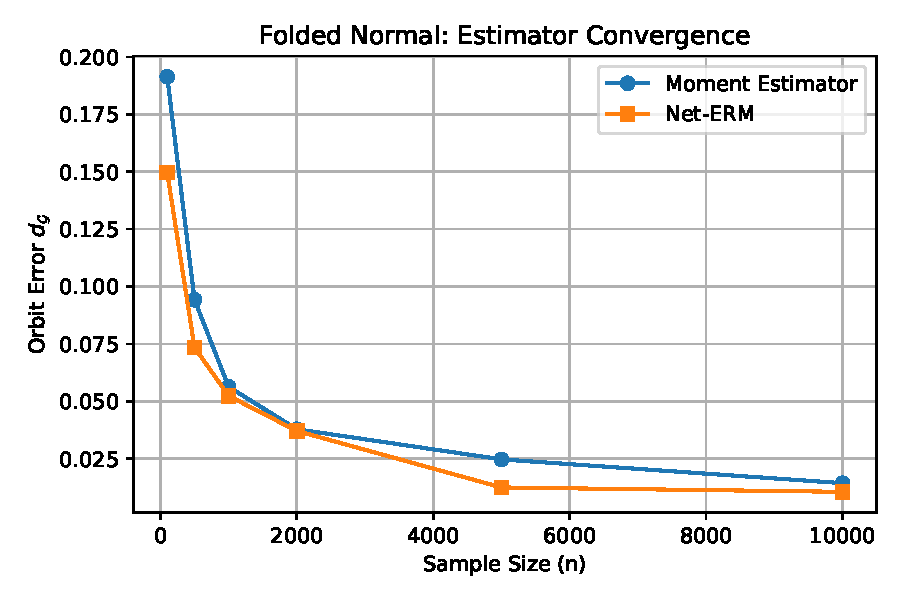
\includegraphics[width=0.48\textwidth]{experiments/folded_normal_py.pdf}
    \hfill
    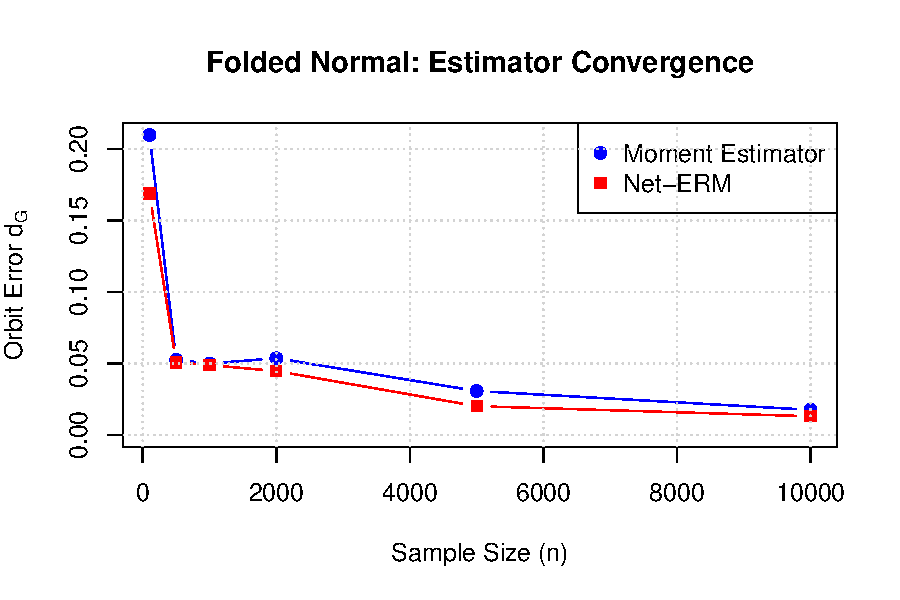
\includegraphics[width=0.48\textwidth]{experiments/folded_normal_r.pdf}
    \caption{Orbit error $\dG$ vs. Sample Size $n$ for the Folded Normal model. Left: Python implementation. Right: R implementation.}
    \label{fig:folded_normal}
\end{figure}

\subsection{Gaussian Mixtures}
For the Gaussian mixture model, we consider a $k=2$ component mixture in 1D with true parameters $w=[0.4, 0.6]$, $\mu=[-2.0, 2.0]$, and $\sigma=[1.0, 1.0]$. The components are identifiable only up to permutation in $\mathfrak{S}_2$.

We evaluate the standard Expectation-Maximization (EM) algorithm as a practical, improper relaxation of the exact Net-ERM, computing the permutation-invariant orbit distance $\dG(\hat\theta, \theta^\star)$. The convergence of the orbit error as $n$ increases is shown in Figure~\ref{fig:gmm_py} (Python) and Figure~\ref{fig:gmm_r} (R).

\begin{figure}[htbp]
    \centering
    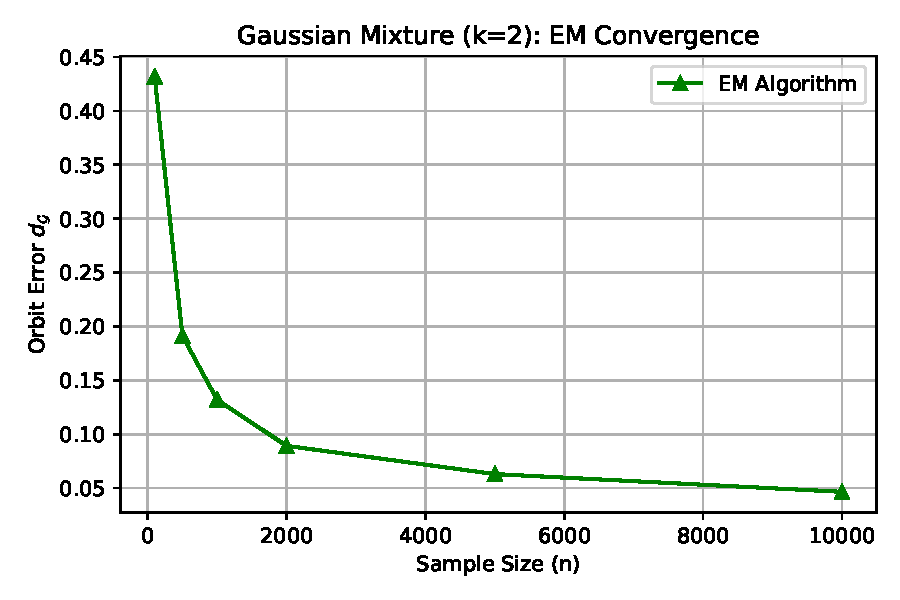
\includegraphics[width=0.48\textwidth]{experiments/gmm_py.pdf}
    \hfill
    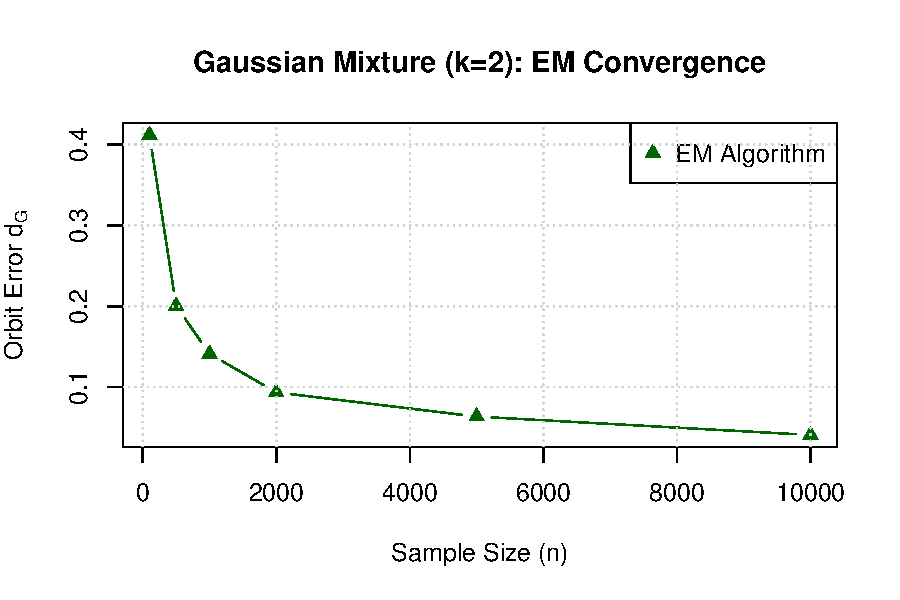
\includegraphics[width=0.48\textwidth]{experiments/gmm_r.pdf}
    \caption{Permutation-invariant orbit error $\dG$ vs. Sample Size $n$ for the $k=2$ Gaussian Mixture model. Left: Python implementation. Right: R implementation.}
    \label{fig:gmm}
\end{figure}

\section{Discussion}
\label{sec:discussion}
We conclude with open problems on sharp minimax rates on quotient spaces and computational-statistical gaps.

\begin{thebibliography}{99}
\bibitem{MallikOrbitHausdorffArxiv}
K.~Mallik,
\emph{Orbit-Hausdorff consistency of maximum likelihood estimators for the folded normal model and finite Gaussian mixtures}.
2025, \href{https://arxiv.org/abs/2509.12206}{\texttt{arXiv:2509.12206}}.

\bibitem{Valiant1984}
L.~G.~Valiant,
A theory of the learnable.
\emph{Commun. ACM} \textbf{27} (1984), no.~11, 1134--1142.

\bibitem{Haussler1992}
D.~Haussler,
Decision theoretic generalizations of the {PAC} model for neural net and other learning applications.
\emph{Inform. Comput.} \textbf{100} (1992), no.~1, 78--150.

\bibitem{ShalevShwartzBenDavid2014}
S.~Shalev-Shwartz and S.~Ben-David,
\emph{Understanding Machine Learning: From Theory to Algorithms}.
Cambridge University Press, 2014.

\bibitem{Tsybakov2009}
A.~B. Tsybakov.
\newblock \emph{Introduction to Nonparametric Estimation}.
\newblock Springer Series in Statistics, Springer, New York, 2009.

\bibitem{Dasgupta1999}
S.~Dasgupta,
Learning mixtures of {Gaussians}.
In \emph{Proc.\ 40th Annual IEEE Symposium on Foundations of Computer Science (FOCS)},
pp.~634--644, 1999.

\bibitem{AroraKannan2001}
S.~Arora and R.~Kannan,
Learning mixtures of arbitrary {Gaussians}.
In \emph{Proc.\ 33rd Annual ACM Symposium on Theory of Computing (STOC)},
pp.~247--257, 2001.

\bibitem{FeldmanServedioODonnell2006}
J.~Feldman, R.~A.~Servedio, and R.~O'Donnell,
{PAC} learning axis-aligned mixtures of {Gaussians} with no separation assumption.
In \emph{Learning Theory (COLT 2006)},
Lecture Notes in Computer Science \textbf{4005}, pp.~20--34,
Springer, 2006.

\bibitem{MoitraValiant2010}
A.~Moitra and G.~Valiant,
Settling the polynomial learnability of mixtures of {Gaussians}.
In \emph{Proc.\ 51st Annual IEEE Symposium on Foundations of Computer Science (FOCS)},
2010.

\bibitem{ToshDasgupta2018}
C.~Tosh and S.~Dasgupta,
Maximum likelihood estimation for mixtures of spherical {Gaussians} is {NP}-hard.
\emph{J. Mach. Learn. Res.} \textbf{18} (2018), no.~175, 1--11.

\bibitem{Teicher1963}
H.~Teicher,
Identifiability of finite mixtures.
\emph{Ann. Math. Statist.} \textbf{34} (1963), no.~4, 1265--1269.

\bibitem{YakowitzSpragins1968}
S.~Yakowitz and J.~D.~Spragins,
On the identifiability of finite mixtures.
\emph{Ann. Math. Statist.} \textbf{39} (1968), no.~1, 209--214.

\bibitem{LeoneNelsonNottingham1961}
F.~C.~Leone, L.~S.~Nelson, and R.~B.~Nottingham,
The folded normal distribution.
\emph{Technometrics} \textbf{3} (1961), no.~4, 543--550.

\bibitem{Elandt1961}
R.~C.~Elandt,
The folded normal distribution: two methods of estimating parameters from moments.
\emph{Technometrics} \textbf{3} (1961), no.~4, 551--562.

\bibitem{Johnson1962}
N.~L.~Johnson,
The folded normal distribution: accuracy of estimation by maximum likelihood.
\emph{Technometrics} \textbf{4} (1962), no.~2, 249--256.

\bibitem{TsagrisBenekiHassani2014}
M.~Tsagris, C.~Beneki, and H.~Hassani,
On the folded normal distribution.
\emph{Mathematics} \textbf{2} (2014), no.~1, 12--28.
\end{thebibliography}

\end{document}
